\documentclass[a4paper,12pt]{article}

\usepackage[utf8]{inputenc}
\usepackage{amsmath}
\usepackage{graphicx}
\usepackage{float}
\usepackage{hyperref}

\title{Relatório sobre Conjuntos, Funções e Operadores Fuzzy}
\author{Doutorado CEFET}
\date{\today}

\begin{document}

\maketitle

\section{Introdução}
Este relatório apresenta a implementação e análise de funções de pertinência, fuzzificação, operações fuzzy e relações fuzzy. As funções de pertinência são amplamente utilizadas em lógica fuzzy para representar graus de pertencimento de elementos a conjuntos fuzzy.

\section{Funções de Pertinência}
\subsection{Implementação de Funcões de Pertinência}

As funções de pertinência implementadas incluem:


\begin{itemize}
    \item Triangular
    \item Trapezoidal
    \item Gaussiana
    \item Sigmoidal
    \item Sinoidal (Bell)
    \item Função S
    \item Função Z
    \item Cauchy
    \item Gaussiana Dupla
    \item Logarítmica
    \item Retangular
\end{itemize}

Para a construção dos gráficos utilizando python utilizamos a função $plot_results$

\begin{verbatim}
def plot_results(x, y, params, type):
    # Plotando a função
    plt.figure(figsize=(8, 5))
    plt.plot(x, y, label=f"{type.capitalize()} {params}")
    plt.title(f"Função {type.capitalize()}")
    plt.xlabel("x")
    plt.ylabel("Grau de Pertinência")
    plt.legend()
    plt.grid()
    plt.savefig(f'{output_dir}/{type}.png')
    plt.show()
\end{verbatim}
    
\subsubsection{Função Triangular}
A função triangular é definida por três parâmetros $(a, b, c)$, onde:
\begin{itemize}
    \item $a$ é o ponto inicial onde a pertinência começa a aumentar;
    \item $b$ é o ponto onde a pertinência atinge o valor máximo (1);
    \item $c$ é o ponto final onde a pertinência retorna a 0.
\end{itemize}
A fórmula é dada por:
\[
\mu(x) =
\begin{cases}
\frac{x - a}{b - a}, & \text{se } a \leq x < b, \\
\frac{c - x}{c - b}, & \text{se } b \leq x < c, \\
0, & \text{caso contrário.}
\end{cases}
\]
O código Python correspondente é:
\begin{verbatim}
def triangular(x, a, b, c):
    if a <= x < b:
        return (x - a) / (b - a)
    elif b <= x < c:
        return (c - x) / (c - b)
    else:
        return 0

# Exemplo de plotagem para a função triangular
a, b, c = 5, 10, 15  # Parâmetros da função triangular
x = np.linspace(0, 20, 100)  # Valores de x no intervalo [0, 20]

# Calcula os graus de pertinência
y = [triangular(val, a, b, c) for val in x]

# Plotando a função triangular
plot_results(x, y, [a, b, c], "triangular")

\end{verbatim}

\begin{figure}[H]
    \centering
    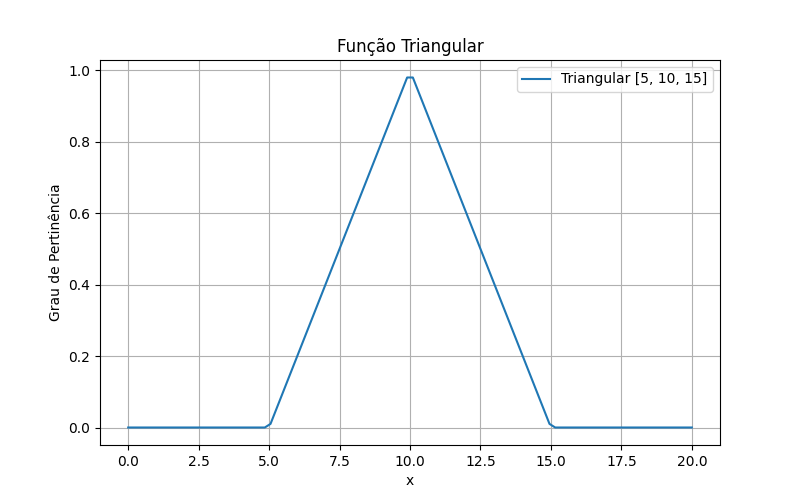
\includegraphics[width=0.8\textwidth]{img/triangular.png}
    \caption{Exemplo de função triangular com $a=5$, $b=10$, $c=15$.}
\end{figure}

\subsubsection{Função Trapezoidal}
A função trapezoidal é definida por quatro parâmetros $(a, b, c, d)$, onde:
\begin{itemize}
    \item $a$ e $d$ são os pontos onde a pertinência é 0;
    \item $b$ e $c$ definem a região onde a pertinência é 1.
\end{itemize}
A fórmula é:
\[
\mu(x) =
\begin{cases}
\frac{x - a}{b - a}, & \text{se } a \leq x < b, \\
1, & \text{se } b \leq x \leq c, \\
\frac{d - x}{d - c}, & \text{se } c < x \leq d, \\
0, & \text{caso contrário.}
\end{cases}
\]
O código Python correspondente é:
\begin{verbatim}
def trapezoidal(x, a, b, c, d):
    if a <= x < b:
        return (x - a) / (b - a)
    elif b <= x <= c:
        return 1
    elif c < x <= d:
        return (d - x) / (d - c)
    else:
        return 0

# Exemplo de plotagem para a função trapezoidal
a, b, c, d = 5, 10, 15, 20  # Parâmetros da função trapezoidal
x = np.linspace(0, 25, 100)  # Valores de x no intervalo [0, 25]

# Calcula os graus de pertinência
y = [trapezoidal(val, a, b, c, d) for val in x]

# Plotando a função trapezoidal
plot_results(x, y, [a, b, c, d], "trapezoidal")

\end{verbatim}
\begin{figure}[H]
    \centering
    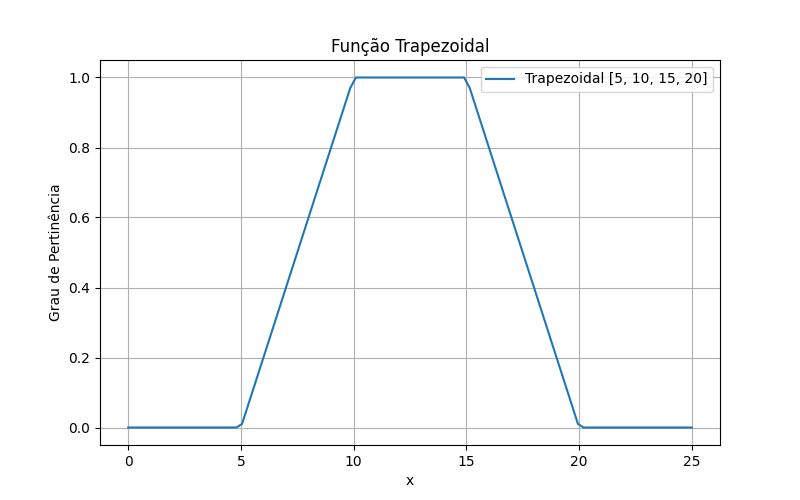
\includegraphics[width=0.8\textwidth]{img/trapezoidal.png}
    \caption{Exemplo de função trapezoidal com $a=5$, $b=10$, $c=15$, $d=20$.}
\end{figure}

\subsubsection{Função Gaussiana}
A função gaussiana é definida por dois parâmetros $(c, \sigma)$, onde:
\begin{itemize}
    \item $c$ é o centro da curva, onde a pertinência é máxima (1);
    \item $\sigma$ controla a largura da curva.
\end{itemize}
A fórmula é:
\[
\mu(x) = e^{-\frac{1}{2} \left( \frac{x - c}{\sigma} \right)^2}.
\]
O código Python correspondente é:
\begin{verbatim}
def gaussian(x, c, sigma):
    return np.exp(-0.5 * ((x - c) / sigma) ** 2)


# Exemplo de uso
x = np.linspace(0, 20, 100)  # Valores de x no intervalo [0, 20]
c = 10  # Centro da curva (onde a pertinência é máxima)
sigma = 3  # Largura da curva

# Calcula os graus de pertinência
y = [gaussian(val, c, sigma) for val in x]

# Plotando a função gaussiana
plot_results(x, y, [c, sigma], "gaussian")
\end{verbatim}
\begin{figure}[H]
    \centering
    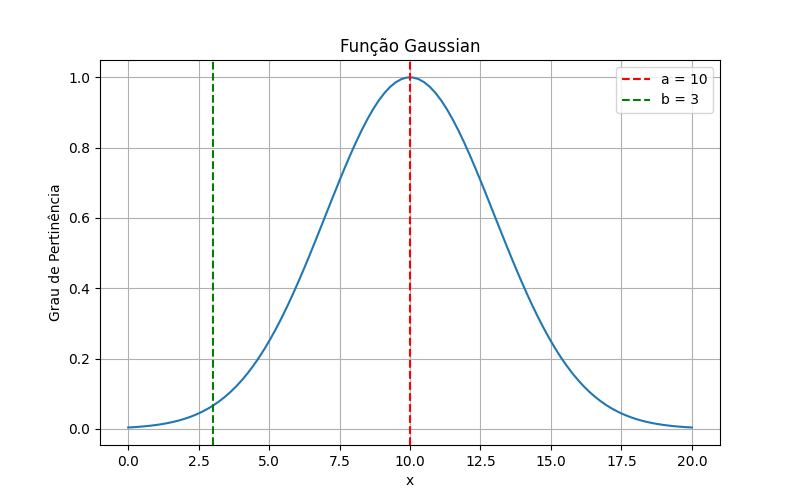
\includegraphics[width=0.8\textwidth]{img/gaussian.png}
    \caption{Exemplo de função gaussiana com $c=10$, $\sigma=3$.}
\end{figure}

\subsubsection{Função Sigmoidal}
A função sigmoidal é definida por dois parâmetros $(a, c)$, onde:
\begin{itemize}
    \item $a$ controla a inclinação da curva;
    \item $c$ é o ponto central onde a pertinência é 0.5.
\end{itemize}
A fórmula é:
\[
\mu(x) = \frac{1}{1 + e^{-a(x - c)}}.
\]
O código Python correspondente é:
\begin{verbatim}
def sigmoidal(x, a, c):
    return 1 / (1 + np.exp(-a * (x - c)))

# Exemplo de plotagem para a função sigmoidal
a, c = 1, 10  # Parâmetros da função sigmoidal
x = np.linspace(0, 20, 100)  # Valores de x no intervalo [0, 20]

# Calcula os graus de pertinência
y = [sigmoidal(val, a, c) for val in x]

# Plotando a função sigmoidal
plot_results(x, y, [a, c], "sigmoidal")
\end{verbatim}

\begin{figure}[H]
    \centering
    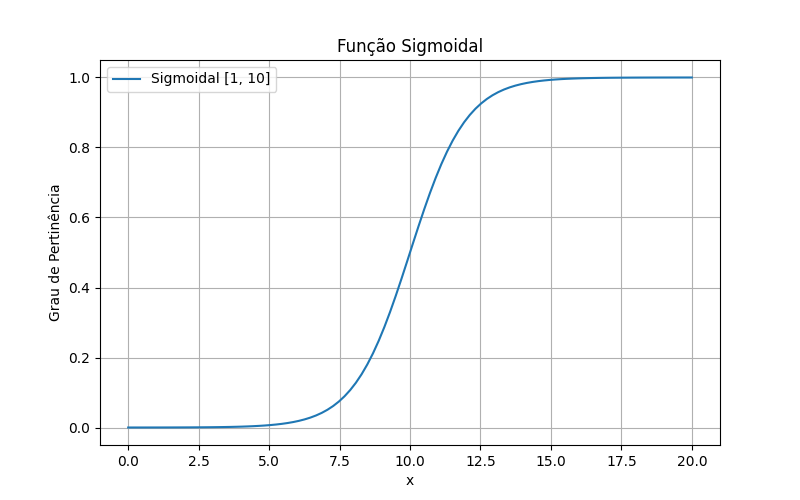
\includegraphics[width=0.8\textwidth]{img/sigmoidal.png}
    \caption{Exemplo de função sigmoidal com $a=1$, $c=10$.}
\end{figure}

\subsubsection{Função Sinoidal (Bell)}
A função Bell é definida por três parâmetros $(a, b, c)$, onde:
\begin{itemize}
    \item $a$ controla a largura da curva;
    \item $b$ controla a inclinação;
    \item $c$ é o centro da curva.
\end{itemize}
A fórmula é:
\[
\mu(x) = \frac{1}{1 + \left|\frac{x - c}{a}\right|^{2b}}.
\]
O código Python correspondente é:
\begin{verbatim}
def bell_function(x, a, b, c):
    return 1 / (1 + abs((x - c) / a) ** (2 * b))
# Exemplo de plotagem para a função Bell
a, b, c = 2, 4, 10  # Parâmetros da função Bell
x = np.linspace(0, 20, 100)  # Valores de x no intervalo [0, 20]

# Calcula os graus de pertinência
y = [bell_function(val, a, b, c) for val in x]

# Plotando a função Bell
plot_results(x, y, [a, b, c], "bell")

\end{verbatim}
\begin{figure}[H]
    \centering
    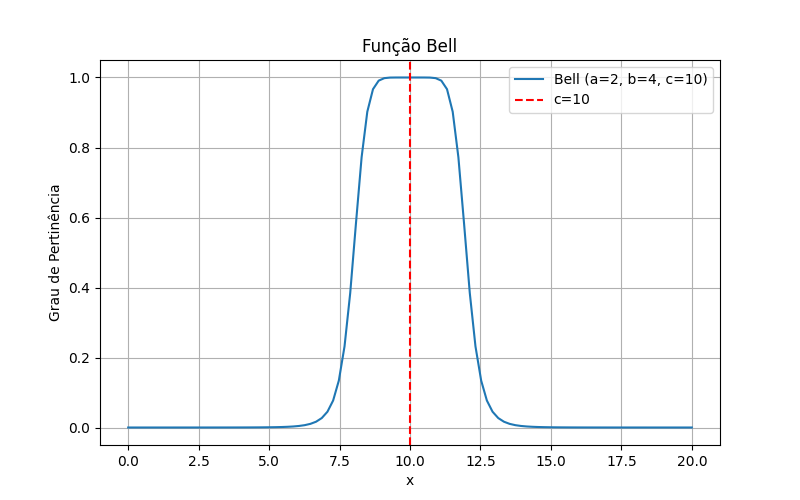
\includegraphics[width=0.8\textwidth]{img/bell.png}
    \caption{Exemplo de função Bell com $a=2$, $b=4$, $c=10$.}
\end{figure}

\subsubsection{Função S}
A função S é definida por dois parâmetros $(a, b)$, onde:
\begin{itemize}
    \item $a$ é o ponto onde a pertinência começa a aumentar;
    \item $b$ é o ponto onde a pertinência atinge 1.
\end{itemize}
A fórmula é:
\[
\mu(x) =
\begin{cases}
0, & \text{se } x \leq a, \\
2\left(\frac{x - a}{b - a}\right)^2, & \text{se } a < x < b, \\
1, & \text{se } x \geq b.
\end{cases}
\]
O código Python correspondente é:
\begin{verbatim}
def s_function(x, a, b):
    if x <= a:
        return 0
    elif a < x < b:
        return 2 * ((x - a) / (b - a)) ** 2
    elif x >= b:
        return 1

# Exemplo de plotagem para a função S
a, b = 5, 15  # Parâmetros da função S
x = np.linspace(0, 20, 100)  # Valores de x no intervalo [0, 20]

# Calcula os graus de pertinência
y = [s_function(val, a, b) for val in x]

# Plotando a função S
plot_results(x, y, [a, b], "s")

\end{verbatim}
\begin{figure}[H]
    \centering
    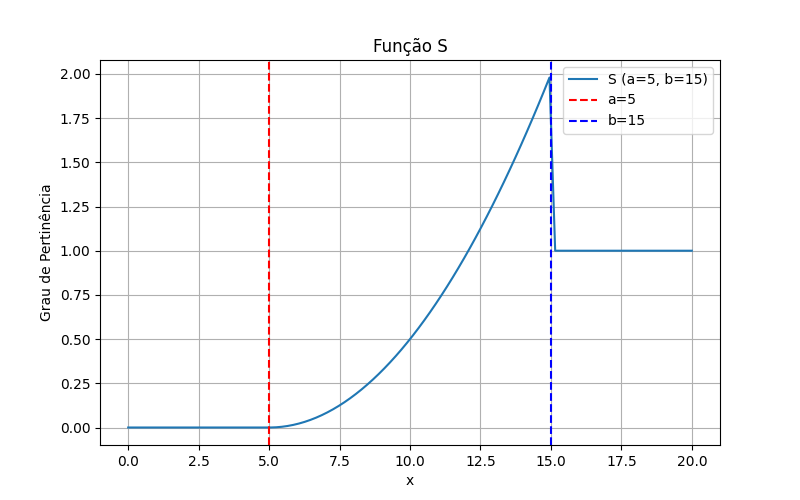
\includegraphics[width=0.8\textwidth]{img/s.png}
    \caption{Exemplo de função S com $a=5$, $b=15$.}
\end{figure}

\subsubsection{Função Z}
A função Z é definida por dois parâmetros $(a, b)$, onde:
\begin{itemize}
    \item $a$ é o ponto onde a pertinência começa a diminuir;
    \item $b$ é o ponto onde a pertinência atinge 0.
\end{itemize}
A fórmula é:
\[
\mu(x) =
\begin{cases}
1, & \text{se } x \leq a, \\
1 - 2\left(\frac{x - a}{b - a}\right)^2, & \text{se } a < x < b, \\
0, & \text{se } x \geq b.
\end{cases}
\]
O código Python correspondente é:
\begin{verbatim}
def z_function(x, a, b):
    if x <= a:
        return 1
    elif a < x < b:
        return 1 - 2 * ((x - a) / (b - a)) ** 2
    else:
        return 0
        
# Exemplo de plotagem para a função Z
a, b = 5, 15  # Parâmetros da função Z
x = np.linspace(0, 20, 100)  # Valores de x no intervalo [0, 20]

# Calcula os graus de pertinência
y = [z_function(val, a, b) for val in x]

# Plotando a função Z
plot_results(x, y, [a, b], "z")


\end{verbatim}

\subsubsection{Função Cauchy}
A função Cauchy é definida por dois parâmetros $(c, \gamma)$, onde:
\begin{itemize}
    \item $c$ é o centro da curva;
    \item $\gamma$ controla a largura da curva.
\end{itemize}
A fórmula é:
\[
\mu(x) = \frac{1}{1 + \left(\frac{x - c}{\gamma}\right)^2}.
\]
O código Python correspondente é:
\begin{verbatim}
def cauchy_function(x, c, gamma):
    return 1 / (1 + ((x - c) / gamma) ** 2)

# Exemplo de plotagem para a função Cauchy
c, gamma = 10, 3  # Parâmetros da função Cauchy
x = np.linspace(0, 20, 100)  # Valores de x no intervalo [0, 20]

# Calcula os graus de pertinência
y = [cauchy_function(val, c, gamma) for val in x]

# Plotando a função Cauchy
plot_results(x, y, [c, gamma], "cauchy")

\end{verbatim}
\begin{figure}[H]
    \centering
    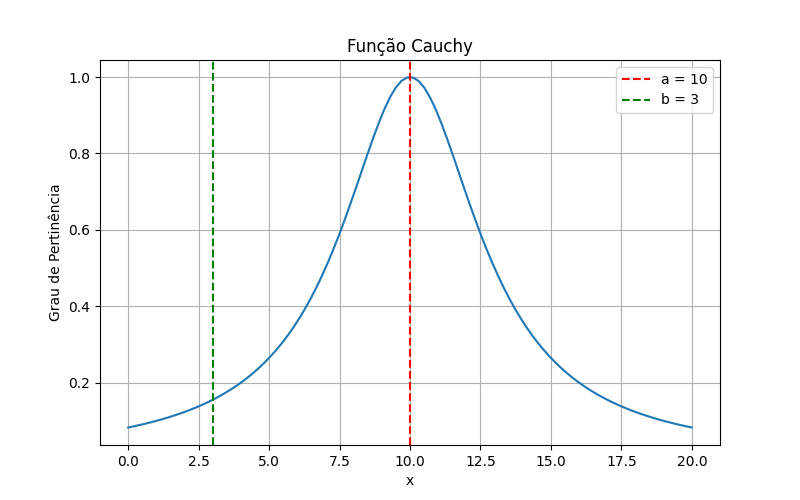
\includegraphics[width=0.8\textwidth]{img/cauchy.png}
    \caption{Exemplo de função Cauchy com $c=10$, $\gamma=3$.}
\end{figure}

\subsubsection{Função Gaussiana Dupla}
A função Gaussiana Dupla é definida por três parâmetros $(c, \sigma_1, \sigma_2)$, onde:
\begin{itemize}
    \item $c$ é o centro da curva;
    \item $\sigma_1$ controla a largura da curva para $x \leq c$;
    \item $\sigma_2$ controla a largura da curva para $x > c$.
\end{itemize}
A fórmula é:
\[
\mu(x) =
\begin{cases}
e^{-\frac{1}{2} \left( \frac{x - c}{\sigma_1} \right)^2}, & \text{se } x \leq c, \\
e^{-\frac{1}{2} \left( \frac{x - c}{\sigma_2} \right)^2}, & \text{se } x > c.
\end{cases}
\]
O código Python correspondente é:
\begin{verbatim}
def double_gaussian(x, c, sigma1, sigma2):
    if x <= c:
        return np.exp(-0.5 * ((x - c) / sigma1) ** 2)
    else:
        return np.exp(-0.5 * ((x - c) / sigma2) ** 2)

# Exemplo de plotagem para a função Gaussiana Dupla
c1, sigma1 = 8, 2  # Parâmetros da primeira gaussiana
c2, sigma2 = 14, 3  # Parâmetros da segunda gaussiana
x = np.linspace(0, 20, 100)  # Valores de x no intervalo [0, 20]

# Calcula os graus de pertinência
y = [double_gaussian(val, c1, sigma1, c2, sigma2) for val in x]

# Plotando a função Gaussiana Dupla
plot_results(x, y, [c1, sigma1, c2, sigma2], "double_gaussian")

\end{verbatim}
\begin{figure}[H]
    \centering
    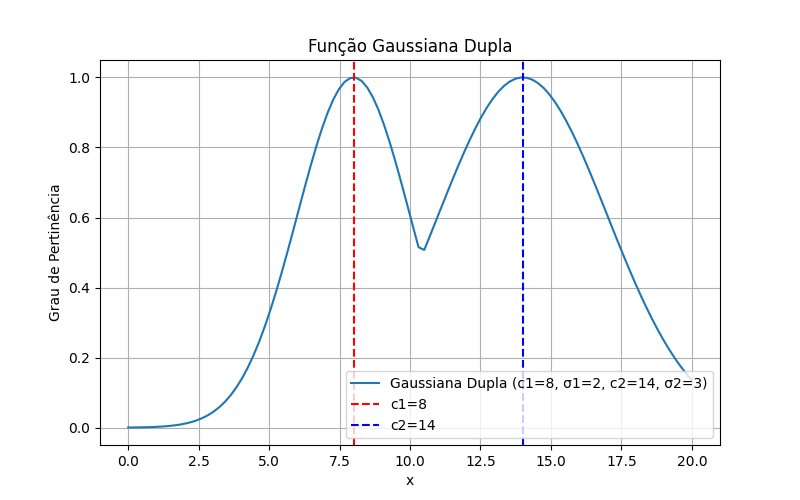
\includegraphics[width=0.8\textwidth]{img/double_gaussian.png}
    \caption{Exemplo de função Gaussiana Dupla com $c=10$, $\sigma_1=3$, $\sigma_2=5$.}
\end{figure}

\subsubsection{Função Retangular}
A função Retangular é definida por dois parâmetros $(a, b)$, onde:
\begin{itemize}
    \item $a$ é o início do intervalo onde a pertinência é 1;
    \item $b$ é o final do intervalo onde a pertinência é 1.
\end{itemize}
A fórmula é:
\[
\mu(x) =
\begin{cases}
1, & \text{se } a \leq x \leq b, \\
0, & \text{caso contrário.}
\end{cases}
\]
O código Python correspondente é:
\begin{verbatim}
def rectangular(x, a, b):
    if a <= x <= b:
        return 1
    else:
        return 0

# Exemplo de plotagem para a função Retangular
a, b = 3, 7  # Parâmetros da função Retangular
x = np.linspace(0, 10, 100)  # Valores de x no intervalo [0, 10]

# Calcula os graus de pertinência
y = [rectangular_function(val, a, b) for val in x]

# Plotando a função Retangular
plot_results(x, y, [a, b], "rectangular")

\end{verbatim}
\begin{figure}[H]
    \centering
    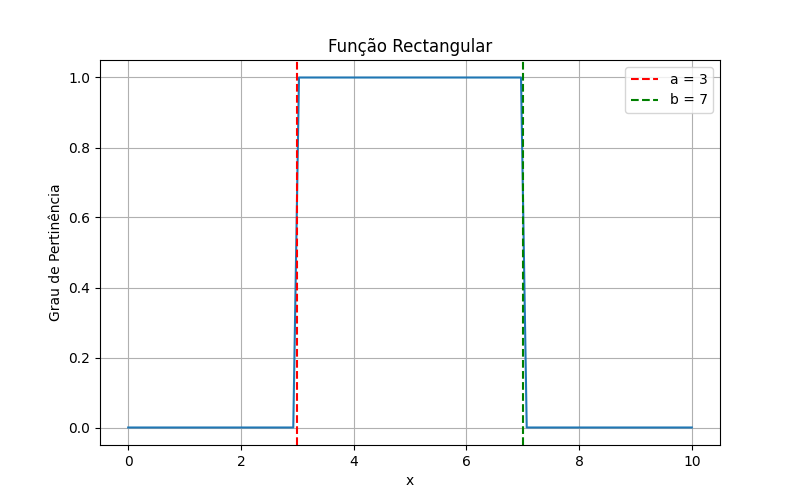
\includegraphics[width=0.8\textwidth]{img/rectangular.png}
    \caption{Exemplo de função Retangular com $a=10$, $b=20$.}
\end{figure}

\subsubsection{Função Logarítmica}
A função Logarítmica é definida por dois parâmetros $(a, b)$, onde:
\begin{itemize}
    \item $a$ controla o deslocamento da curva;
    \item $b$ controla a inclinação da curva.
\end{itemize}
A fórmula é:
\[
\mu(x) = 
\begin{cases}
0, & \text{se } x \leq a, \\
\log_b(x - a + 1), & \text{se } x > a.
\end{cases}
\]
O código Python correspondente é:
\begin{verbatim}
import math

def logarithmic_function(x, a, b):
    if x <= a:
        return 0
    else:
        return math.log(x - a + 1, b)

# Exemplo de plotagem para a função Logarítmica
a, b = 2, 1  # Parâmetros da função Logarítmica
x = np.linspace(0.1, 10, 100)  # Valores de x no intervalo [0.1, 10] (evitando zero)

# Calcula os graus de pertinência
y = [logarithmic_function(val, a, b) for val in x]

# Plotando a função Logarítmica
plot_results(x, y, [a, b], "logarithmic")
\end{verbatim}
\begin{figure}[H]
    \centering
    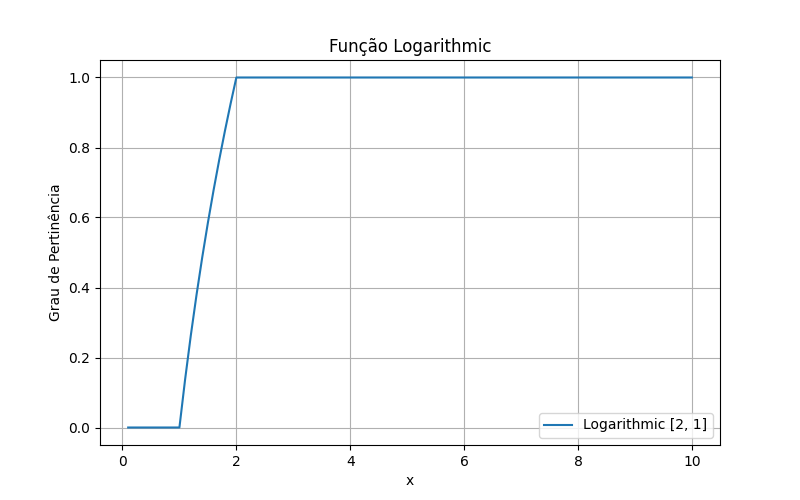
\includegraphics[width=0.8\textwidth]{img/logarithmic.png}
    \caption{Exemplo de função Logarítmica com $a=5$, $b=2$.}
\end{figure}


\subsection{Fuzzificação e Análise Comparativa}
Para a fuzzificação, escolhemos uma variável de entrada com universo de discurso definido e particionamos o domínio em funções de pertinência uniformemente espaçadas. A seguir, apresentamos os resultados para duas amostras distintas.

Para as variáveis de entrada definir um universo de estudo como segue, particionado esse domínio em quatro funções de pertinência uniformemente espaçadas. 

\begin{itemize}
    \item **Frio**: Representa temperaturas baixas, variando de $0$ a aproximadamente $25$ graus.
    \item **Morno**: Temperatura intermediária, abrangendo valores entre $20$ e $50$ graus.
    \item **Quente**: Engloba valores de temperatura entre $45$ e $75$ graus.
    \item **Muito Quente**: Abrange temperaturas elevadas, variando de $70$ a $100$ graus.
\end{itemize}

Para realizar o espaçamento fizemos o algoritmo que se segue onde retorna os parametros: 


\begin{verbatim}
def generate_params(X, types, n):
    centers = np.linspace(X[0], X[1], n)  # Centros uniformemente distribuídos
    step = (X[1] - X[0]) / (n - 1) if n > 1 else (X[1] - X[0])  # Espaçamento entre os centros
    params = []

    for i, t in enumerate(types):
        if t == 'gaussian':
            sigma = step / 2  # Sigma proporcional ao espaçamento
            params.append([centers[i], sigma])
        elif t == 'triangular':
            a = max(X[0], centers[i] - step)  # Início da base
            b = centers[i]                   # Pico
            c = min(X[1], centers[i] + step)  # Fim da base
            params.append([a, b, c])
        elif t == 'trapezoidal':
            a = max(X[0], centers[i] - step)  # Início da base
            b = max(X[0], centers[i] - step / 2)  # Início do topo
            c = min(X[1], centers[i] + step / 2)  # Fim do topo
            d = min(X[1], centers[i] + step)  # Fim da base
            params.append([a, b, c, d])
        elif t == 'sigmoidal':
            a = 1  # Inclinação padrão
            c = centers[i]  # Centro
            params.append([a, c])
        elif t == 'bell':
            a = step / 2  # Largura do sino
            b = 2  # Inclinação padrão
            c = centers[i]  # Centro
            params.append([a, b, c])
        elif t == 'z':
            a = max(X[0], centers[i] - step)  # Início do decaimento
            b = centers[i]  # Fim do decaimento
            params.append([a, b])
        elif t == 's':
            a = centers[i]  # Início do crescimento
            b = min(X[1], centers[i] + step)  # Fim do crescimento
            params.append([a, b])
       
        elif t == 'cauchy':
            c = centers[i]  # Centro
            gamma = step / 2  # Largura
            params.append([c, gamma])
        elif t == 'double_gaussian':
            c1 = max(X[0], centers[i] - step / 2)  # Centro da primeira gaussiana
            sigma1 = step / 4  # Largura da primeira gaussiana
            c2 = min(X[1], centers[i] + step / 2)  # Centro da segunda gaussiana
            sigma2 = step / 4  # Largura da segunda gaussiana
            params.append([c1, sigma1, c2, sigma2])
        elif t == 'retangular':
            a = max(X[0], centers[i] - step / 2)  # Início do intervalo
            b = min(X[1], centers[i] + step / 2)  # Fim do intervalo
            params.append([a, b])
        elif t == 'linear':  # Adicionando a função linear
            a = max(X[0], centers[i] - step)  # Início da base
            b = min(X[1], centers[i] + step)  # Fim da base
            params.append([a, b])
        else:
            raise ValueError(f"Tipo de função de pertinência'{t}' não suportado!")
    
    return params
\end{verbatim}


Outra função e para calcular o graus de pertinência para cada atributo, nesse algortmo esolhemos as funções de pertinência relacionadas a seção 2. 

\begin{verbatim}
### Função Membership
def calculate_membership(dominio, types, params):
    x = np.linspace(dominio[0], dominio[1], 100)  # Gera os valores de x no domínio
    results = []
    for func_type, func_params in zip(types, params):
        
        # Calcula os graus de pertinência com base no tipo de função
        if func_type == 'linear':
            results.append([linear_function(val, *func_params) for val in x])  
        elif func_type == 'triangular':
            results.append([triangular(val, *func_params) for val in x])
        elif func_type == 'trapezoidal':
            results.append([trapezoidal(val, *func_params) for val in x])
        elif func_type == 'gaussian':
            results.append([gaussian(val, *func_params) for val in x])
        elif func_type == 'sigmoidal':
            results.append([sigmoidal(val, *func_params) for val in x])
        elif func_type == 'z':
            results.append([z_function(val, *func_params) for val in x])
        elif func_type == 's':
            results.append([s_function(val, *func_params) for val in x])
        elif func_type == 'pi':
            results.append([pi_function(val, *func_params) for val in x])
        elif func_type == 'bell':
            results.append([bell_function(val, *func_params) for val in x])
        elif func_type == 'singleton':
            results.append([singleton_function(val, *func_params) for val in x])
        elif func_type == 'cauchy':
            results.append([cauchy_function(val, *func_params) for val in x])
        elif func_type == 'double_gaussian':
            results.append([double_gaussian(val, *func_params) for val in x])
        elif func_type == 'retangular':
            results.append([rectangular_function(val, *func_params) for val in x])
        elif func_type == 'logaritmica':
            results.append([logarithmic_function(val, *func_params) for val in x])
        else:
            raise ValueError(f"Tipo de função desconhecido: {func_type}")

    return x, results
\end{verbatim}


Para a lotagem dos graficos usamos a função 
\begin{verbatim}
def plot_membership_with_samples(x, results, labels, samples, title, activations):
    plt.figure(figsize=(10, 6))
    for j, sample in enumerate(samples):
            # Adiciona uma linha vertical para cada amostra
            random_color = np.random.rand(3,)
            plt.axvline(sample, color=random_color, linestyle='--', alpha=0.7, label=f"Sample: {sample}")
    for i, result in enumerate(results):
        # Plota a função de pertinência com o rótulo correspondente
        plt.plot(x, result, label=f"{labels[i]}")
        for j, sample in enumerate(samples):
           
            # Pega o grau de ativação correspondente
            activation = activations[i][j]
            # Adiciona um ponto no gráfico para destacar a ativação
            random_color = np.random.rand(3,)
            plt.scatter(sample, activation, color=random_color, 
                        label=f"Sample {sample}: {activation:.2f}")

    # Configurações do gráfico
    plt.title(title)
    plt.xlabel("x")
    plt.ylabel("Grau de Pertinência")
    plt.legend(loc="upper right", bbox_to_anchor=(1.3, 1), title="Funções Fuzzy")
    plt.grid()
    plt.tight_layout()
    plt.savefig(f'{output_dir}/{title.replace("- ", "").lower().replace(" ", "_")}_fuzzificado.png')  # Salva o gráfico
    plt.show()
\end{verbatim}

Por fim construir a função fuzificação 
\begin{verbatim}
    def fuzzificacao(n, type, dominio, samples, labels, liguistica):
    # Número de funções de pertinência para cada atributo
    types = [type] * n

    # Geração dos parâmetros para cada tipo de função
    params = generate_params(dominio, types, n)

    for i in range(n):
        v = dominio[1] - dominio[0]  # Tamanho do intervalo
        p = v / n  # Espaçamento correto entre os pontos
        intervalo = [round(dominio[0] + p * i, 2), round(dominio[0] + p * (i + 1), 2)]
        parametros_formatados = [float(round(val, 2)) for val in params[i]]


        print(f'{labels[i]}: {liguistica} - {intervalo} - Parâmetros: {parametros_formatados}')
    # Cálculo dos graus de pertinência para cada atributo
    x, results = calculate_membership(dominio, types, params)
    # Cálculo do grau de ativação para cada amostra
    activations = []
    for i, result in enumerate(results):
        sample_activations = []
        for sample in samples:
            # Encontra o índice mais próximo do valor da amostra no domínio
            idx = np.abs(x - sample).argmin()
            activation = result[idx]
            sample_activations.append(activation)
        activations.append(sample_activations)

    # Imprime as ativações calculadas com melhor formatação
    print(f"\nAtivações para o tipo {type}:")
    print(f"Samples: {samples}")
    for i, sample_activations in enumerate(activations):
         # Arredonda os valores para duas casas decimais
        rounded_activations = np.round(sample_activations, 2)
        print(f"{labels[i]}: {rounded_activations.tolist()}")

    # Plotagem das funções de pertinência para o atributo com as amostras
    plot_membership_with_samples(
        x, results, labels, samples, f"Funções de Pertinência - {type}", activations
    )

\end{verbatim}

com todas as função feitas definir o exemplo: 

\begin{verbatim}
    # Definição do universo de discurso
    dominio = (0, 100)  # Intervalo do universo de discurso
    samples = [25, 75]  # Amostras para fuzzificação
    n = 5
    linguistica = 'temperatura'
    funcao_pertinecia = [
        'triangular', 'trapezoidal', 'gaussian', 'sigmoidal', 'bell', 's', 'z', 'cauchy', 'double_gaussian', 'retangular', 'linear'
    ]
    
    labels = ['Muito Firo', 'Frio', 'Morno', 'Quente', 'Muito quente']
    
    for type in funcao_pertinecia:
        
        fuzzificacao(n, type  , dominio, samples, [labels[i] for i in range(n)], linguistica)
    
    
\end{verbatim}

dominio = (0, 100) 
samples = [25, 75]


\subsubsection{Função Triangular}
Muito Firo: temperatura - [0.0, 20.0] - Parâmetros: [0.0, 0.0, 25.0]
Frio: temperatura - [20.0, 40.0] - Parâmetros: [0.0, 25.0, 50.0]
Morno: temperatura - [40.0, 60.0] - Parâmetros: [25.0, 50.0, 75.0]
Quente: temperatura - [60.0, 80.0] - Parâmetros: [50.0, 75.0, 100.0]
Muito quente: temperatura - [80.0, 100.0] - Parâmetros: [75.0, 100.0, 100.0]

Ativações para o tipo triangular:
Samples: [25, 75]
Muito Firo: [0, 0]
Frio: [0.99, 0.0]
Morno: [0.01, 0.01]
Quente: [0.0, 0.99]
Muito quente: [0, 0]


\begin{figure}[H]
    \centering
    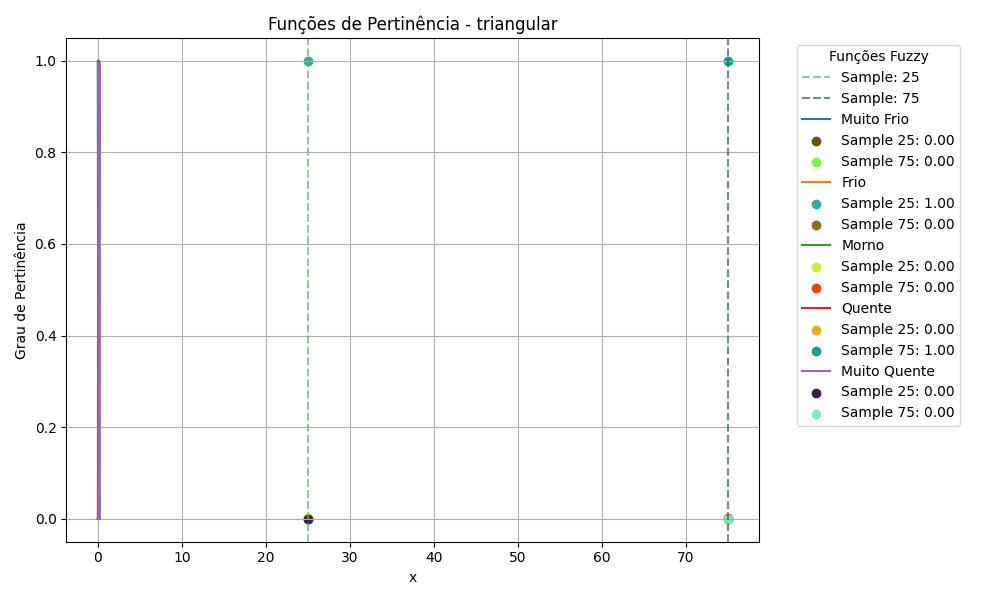
\includegraphics[width=0.8\textwidth]{img/funções_de_pertinência_triangular_fuzzificado.png}
    \caption{Funções de pertinência triangulares e graus de ativação.}
\end{figure}

\subsubsection{Função Trapezoidal}

Muito Firo: temperatura - [0.0, 20.0] - Parâmetros: [0.0, 0.0, 12.5, 25.0]
Frio: temperatura - [20.0, 40.0] - Parâmetros: [0.0, 12.5, 37.5, 50.0]
Morno: temperatura - [40.0, 60.0] - Parâmetros: [25.0, 37.5, 62.5, 75.0]
Quente: temperatura - [60.0, 80.0] - Parâmetros: [50.0, 62.5, 87.5, 100.0]
Muito quente: temperatura - [80.0, 100.0] - Parâmetros: [75.0, 87.5, 100.0, 100.0]


\begin{figure}[H]
    \centering
    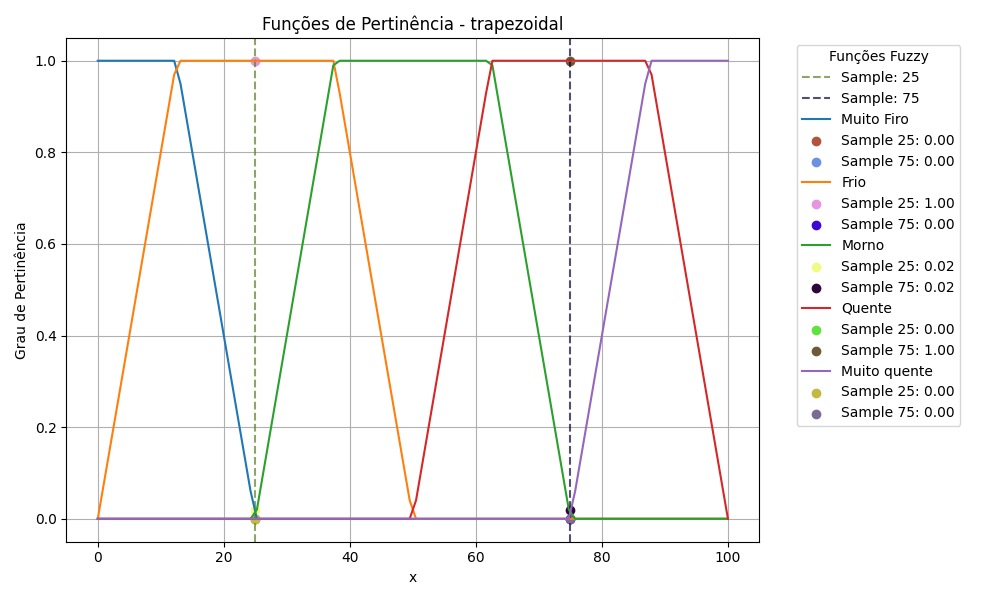
\includegraphics[width=0.8\textwidth]{img/funções_de_pertinência_trapezoidal_fuzzificado.png}
    \caption{Funções de pertinência trapezoidais e graus de ativação.}
\end{figure}

Ativações para o tipo trapezoidal:
Samples: [25, 75]
Muito Firo: [0, 0]
Frio: [1, 0]
Morno: [0.02, 0.02]
Quente: [0, 1]
Muito quente: [0, 0]

\subsubsection{Função Gaussiana}
Muito Firo: temperatura - [0.0, 20.0] - Parâmetros: [0.0, 12.5]
Frio: temperatura - [20.0, 40.0] - Parâmetros: [25.0, 12.5]
Morno: temperatura - [40.0, 60.0] - Parâmetros: [50.0, 12.5]
Quente: temperatura - [60.0, 80.0] - Parâmetros: [75.0, 12.5]
Muito quente: temperatura - [80.0, 100.0] - Parâmetros: [100.0, 12.5]

\begin{figure}[H]
    \centering
    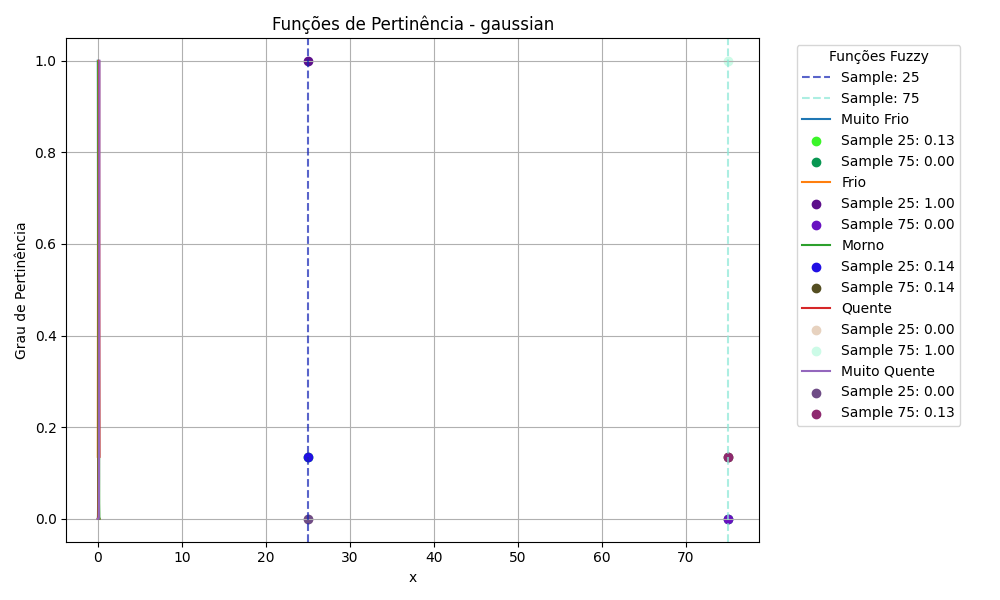
\includegraphics[width=0.8\textwidth]{img/funções_de_pertinência_gaussian_fuzzificado.png}
    \caption{Funções de pertinência gaussianas e graus de ativação.}
\end{figure}

Samples: [25, 75]
Muito Firo: [0.13, 0.0]
Frio: [1.0, 0.0]
Morno: [0.14, 0.14]
Quente: [0.0, 1.0]
Muito quente: [0.0, 0.13]

\subsubsection{Função Sigmoidal}

Muito Firo: temperatura - [0.0, 20.0] - Parâmetros: [1.0, 0.0]
Frio: temperatura - [20.0, 40.0] - Parâmetros: [1.0, 25.0]
Morno: temperatura - [40.0, 60.0] - Parâmetros: [1.0, 50.0]
Quente: temperatura - [60.0, 80.0] - Parâmetros: [1.0, 75.0]
Muito quente: temperatura - [80.0, 100.0] - Parâmetros: [1.0, 100.0]

\begin{figure}[H]
    \centering
    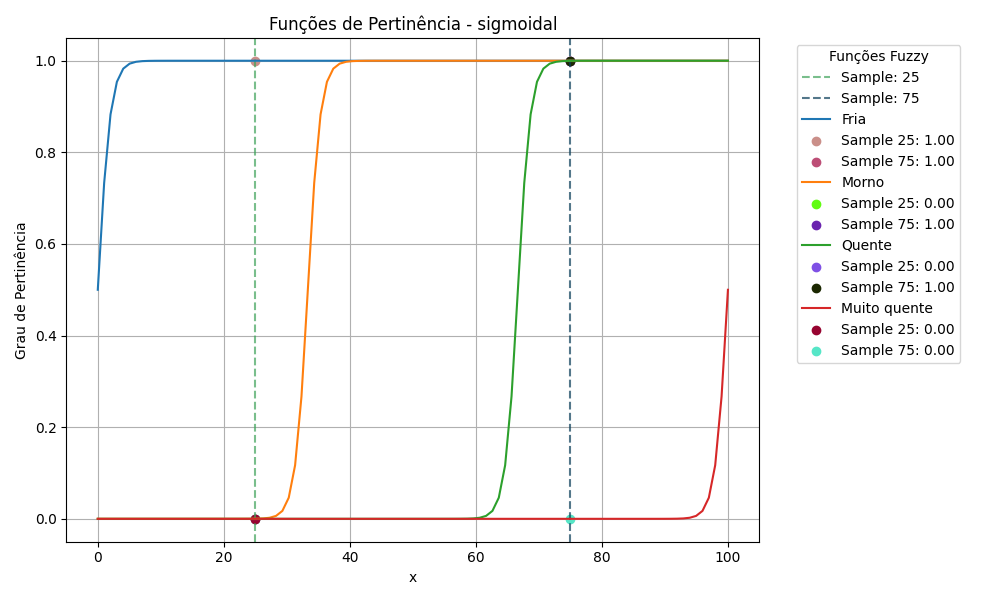
\includegraphics[width=0.8\textwidth]{img/funções_de_pertinência_sigmoidal_fuzzificado.png}
    \caption{Funções de pertinência sigmoidais e graus de ativação.}
\end{figure}
Ativações para o tipo gaussian:

Ativações para o tipo sigmoidal:
Samples: [25, 75]
Muito Firo: [1.0, 1.0]
Frio: [0.56, 1.0]
Morno: [0.0, 1.0]
Quente: [0.0, 0.44]
Muito quente: [0.0, 0.0]


\subsubsection{Função Bell}

Muito Firo: temperatura - [0.0, 20.0] - Parâmetros: [12.5, 2.0, 0.0]
Frio: temperatura - [20.0, 40.0] - Parâmetros: [12.5, 2.0, 25.0]
Morno: temperatura - [40.0, 60.0] - Parâmetros: [12.5, 2.0, 50.0]
Quente: temperatura - [60.0, 80.0] - Parâmetros: [12.5, 2.0, 75.0]
Muito quente: temperatura - [80.0, 100.0] - Parâmetros: [12.5, 2.0, 100.0]

\begin{figure}[H]
    \centering
    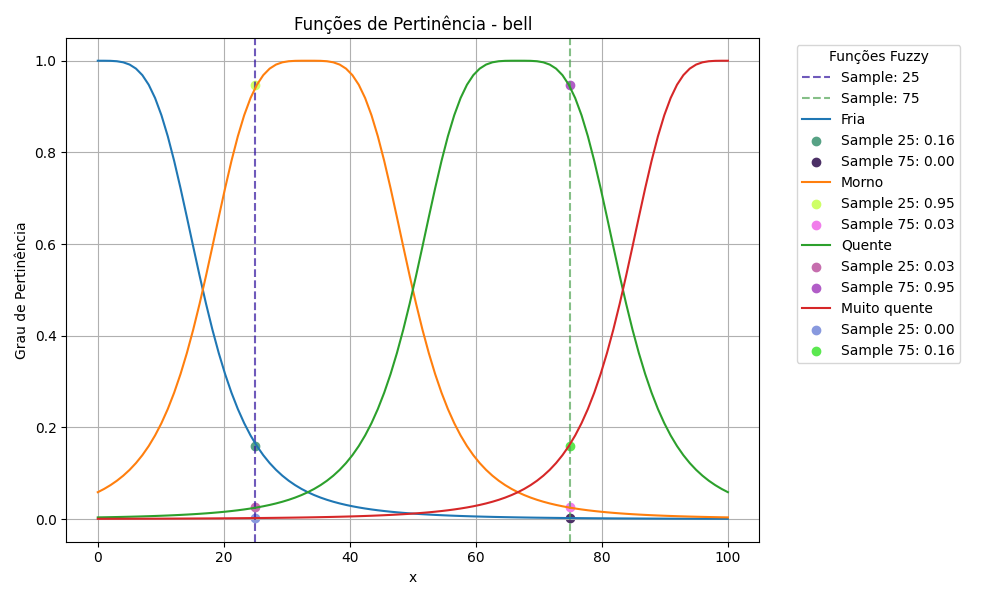
\includegraphics[width=0.8\textwidth]{img/funções_de_pertinência_bell_fuzzificado.png}
    \caption{Funções de pertinência sigmoidais e graus de ativação.}
\end{figure}
Ativações para o tipo gaussian:

Ativações para o tipo bell:
Samples: [25, 75]
Muito Firo: [0.06, 0.0]
Frio: [1.0, 0.0]
Morno: [0.06, 0.06]
Quente: [0.0, 1.0]
Muito quente: [0.0, 0.06]


\subsubsection{Função S}

Muito Firo: temperatura - [0.0, 20.0] - Parâmetros: [0.0, 25.0]
Frio: temperatura - [20.0, 40.0] - Parâmetros: [25.0, 50.0]
Morno: temperatura - [40.0, 60.0] - Parâmetros: [50.0, 75.0]
Quente: temperatura - [60.0, 80.0] - Parâmetros: [75.0, 100.0]
Muito quente: temperatura - [80.0, 100.0] - Parâmetros: [100.0, 100.0]


Quente: [0, 0]
Muito quente: [0, 0]

\begin{figure}[H]
    \centering
    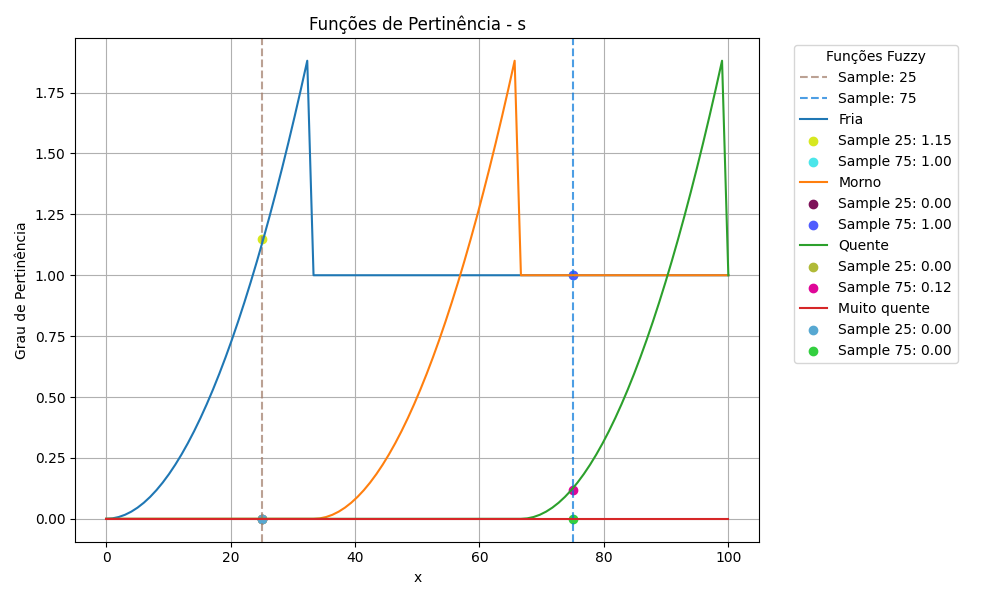
\includegraphics[width=0.8\textwidth]{img/funções_de_pertinência_s_fuzzificado.png}
    \caption{Funções de pertinência sigmoidais e graus de ativação.}
\end{figure}
Ativações para o tipo gaussian:

Ativações para o tipo s:
Samples: [25, 75]
Muito Firo: [1, 1]
Frio: [0.0, 1.0]
Morno: [0.0, 1.96]

\subsubsection{Função S}

Muito Firo: temperatura - [0.0, 20.0] - Parâmetros: [0.0, 25.0]
Frio: temperatura - [20.0, 40.0] - Parâmetros: [25.0, 50.0]
Morno: temperatura - [40.0, 60.0] - Parâmetros: [50.0, 75.0]
Quente: temperatura - [60.0, 80.0] - Parâmetros: [75.0, 100.0]
Muito quente: temperatura - [80.0, 100.0] - Parâmetros: [100.0, 100.0]

\begin{figure}[H]
    \centering
    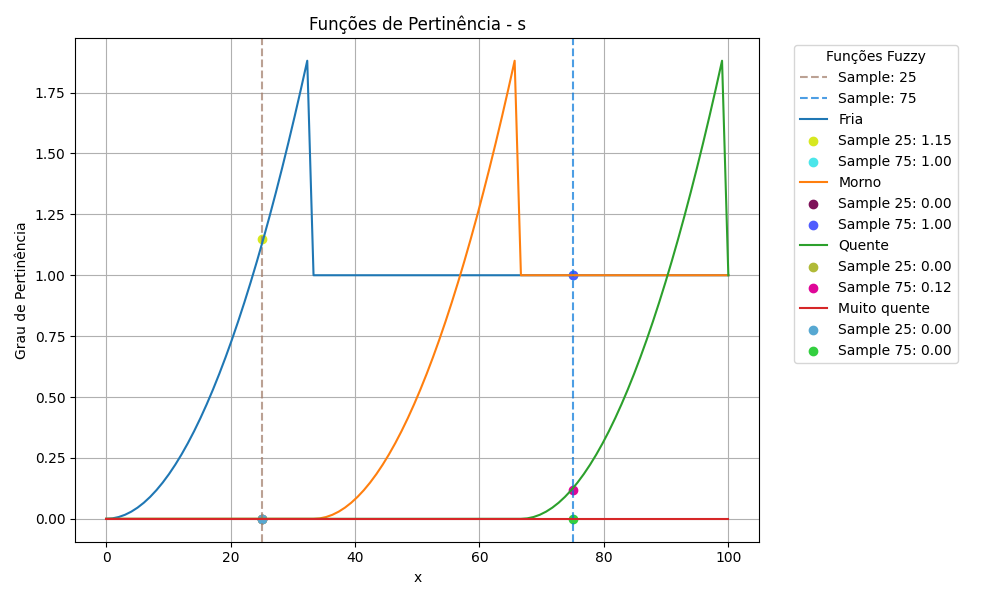
\includegraphics[width=0.8\textwidth]{img/funções_de_pertinência_s_fuzzificado.png}
    \caption{Funções de pertinência sigmoidais e graus de ativação.}
\end{figure}
Ativações para o tipo gaussian:

Ativações para o tipo s:
Samples: [25, 75]
Muito Firo: [1, 1]
Frio: [0.0, 1.0]
Morno: [0.0, 1.96]
Quente: [0, 0]
Muito quente: [0, 0]

\subsubsection{Função Z}

Muito Firo: temperatura - [0.0, 20.0] - Parâmetros: [0.0, 0.0]
Frio: temperatura - [20.0, 40.0] - Parâmetros: [0.0, 25.0]
Morno: temperatura - [40.0, 60.0] - Parâmetros: [25.0, 50.0]
Quente: temperatura - [60.0, 80.0] - Parâmetros: [50.0, 75.0]
Muito quente: temperatura - [80.0, 100.0] - Parâmetros: [75.0, 100.0]

\begin{figure}[H]
    \centering
    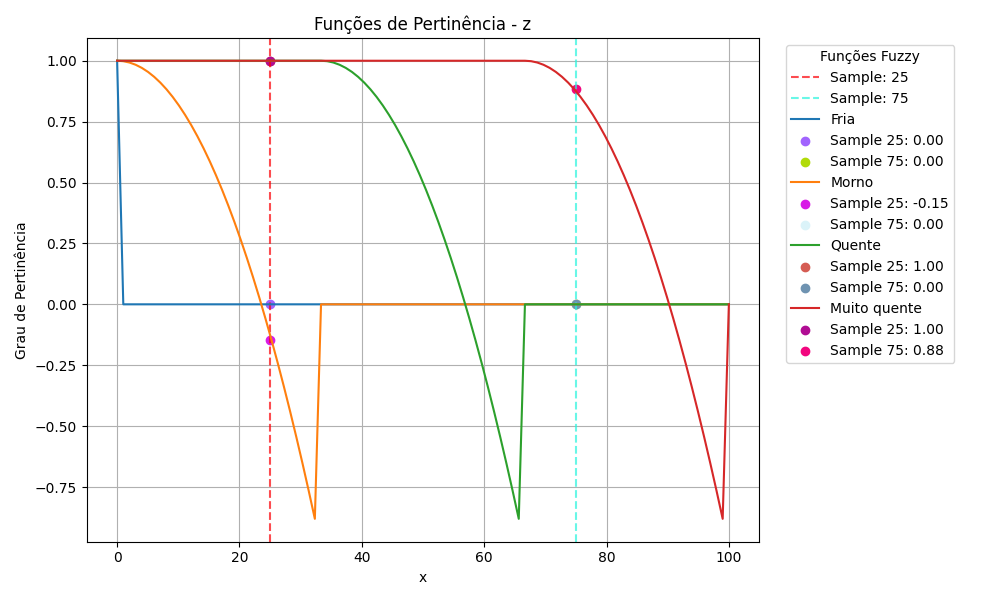
\includegraphics[width=0.8\textwidth]{img/funções_de_pertinência_z_fuzzificado.png}
    \caption{Funções de pertinência sigmoidais e graus de ativação.}
\end{figure}
Ativações para o tipo gaussian:

Ativações para o tipo z:
Samples: [25, 75]
Muito Firo: [0, 0]
Frio: [0, 0]
Morno: [1.0, 0.0]
Quente: [1.0, -0.96]
Muito quente: [1, 1]

\subsubsection{Função Cauchy}

Muito Firo: temperatura - [0.0, 20.0] - Parâmetros: [0.0, 12.5]
Frio: temperatura - [20.0, 40.0] - Parâmetros: [25.0, 12.5]
Morno: temperatura - [40.0, 60.0] - Parâmetros: [50.0, 12.5]
Quente: temperatura - [60.0, 80.0] - Parâmetros: [75.0, 12.5]
Muito quente: temperatura - [80.0, 100.0] - Parâmetros: [100.0, 12.5]

\begin{figure}[H]
    \centering
    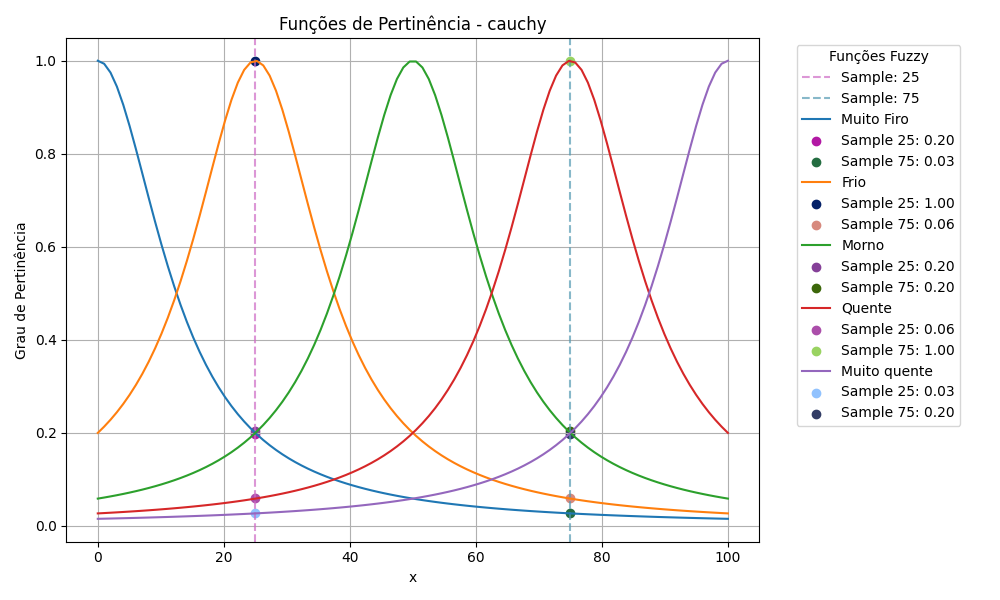
\includegraphics[width=0.8\textwidth]{img/funções_de_pertinência_cauchy_fuzzificado.png}
    \caption{Funções de pertinência sigmoidais e graus de ativação.}
\end{figure}
Ativações para o tipo gaussian:

Ativações para o tipo cauchy:
Samples: [25, 75]
Muito Firo: [0.2, 0.03]
Frio: [1.0, 0.06]
Morno: [0.2, 0.2]
Quente: [0.06, 1.0]
Muito quente: [0.03, 0.2]

\subsubsection{Função Gaussiana Dupla}

Muito Firo: temperatura - [0.0, 20.0] - Parâmetros: [0.0, 6.25, 12.5, 6.25]
Frio: temperatura - [20.0, 40.0] - Parâmetros: [12.5, 6.25, 37.5, 6.25]
Morno: temperatura - [40.0, 60.0] - Parâmetros: [37.5, 6.25, 62.5, 6.25]
Quente: temperatura - [60.0, 80.0] - Parâmetros: [62.5, 6.25, 87.5, 6.25]
Muito quente: temperatura - [80.0, 100.0] - Parâmetros: [87.5, 6.25, 100.0, 6.25]

\begin{figure}[H]
    \centering
    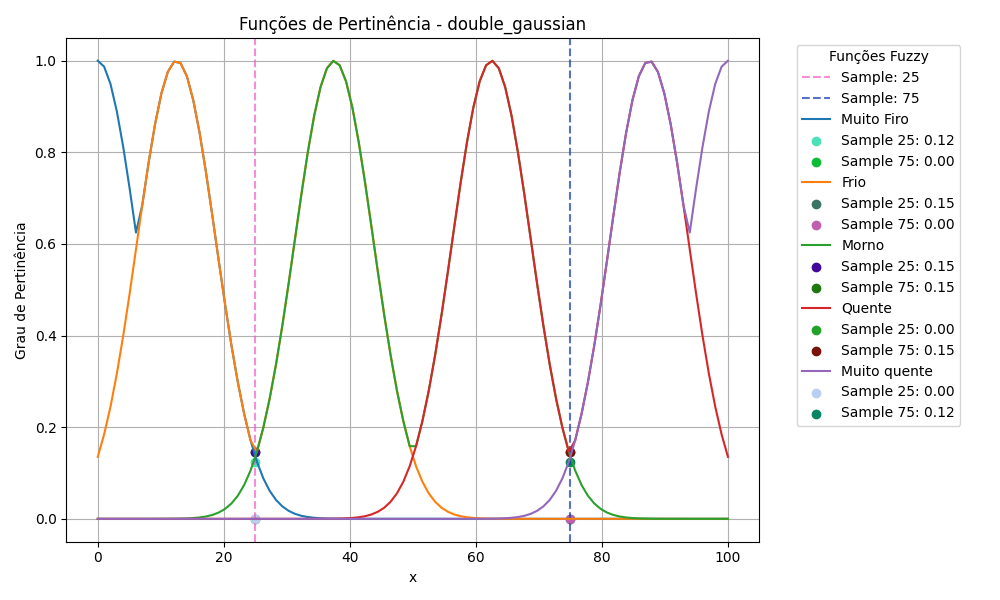
\includegraphics[width=0.8\textwidth]{img/funções_de_pertinência_double_gaussian_fuzzificado.png}
    \caption{Funções de pertinência sigmoidais e graus de ativação.}
\end{figure}
Ativações para o tipo gaussian:

Ativações para o tipo double gaussian:
Samples: [25, 75]
Muito Firo: [0.12, 0.0]
Frio: [0.15, 0.0]
Morno: [0.15, 0.15]
Quente: [0.0, 0.15]
Muito quente: [0.0, 0.12]

\subsubsection{Função Retangular}

Muito Firo: temperatura - [0.0, 20.0] - Parâmetros: [0.0, 12.5]
Frio: temperatura - [20.0, 40.0] - Parâmetros: [12.5, 37.5]
Morno: temperatura - [40.0, 60.0] - Parâmetros: [37.5, 62.5]
Quente: temperatura - [60.0, 80.0] - Parâmetros: [62.5, 87.5]
Muito quente: temperatura - [80.0, 100.0] - Parâmetros: [87.5, 100.0]

\begin{figure}[H]
    \centering
    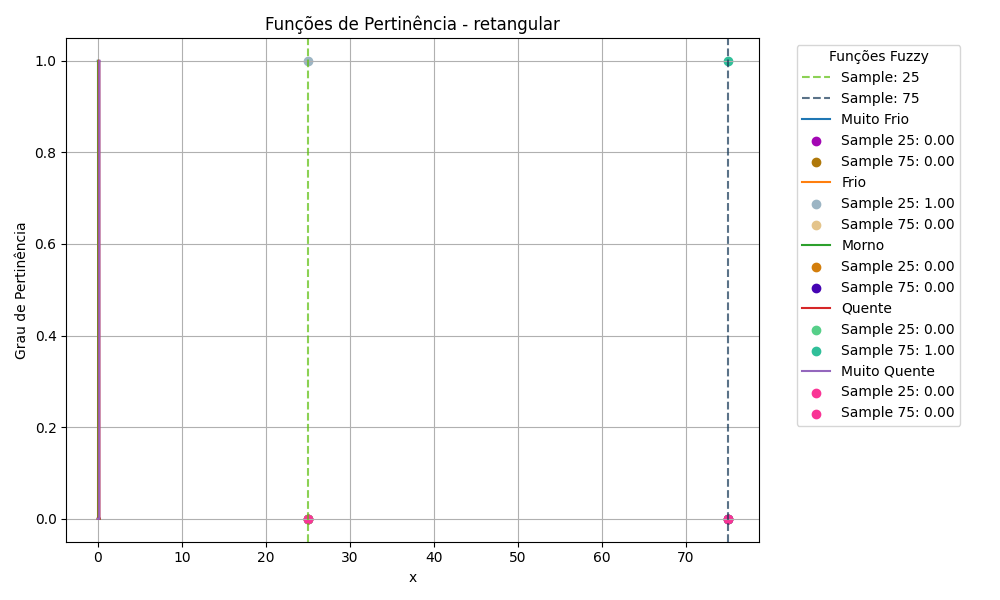
\includegraphics[width=0.8\textwidth]{img/funções_de_pertinência_retangular_fuzzificado.png}
    \caption{Funções de pertinência sigmoidais e graus de ativação.}
\end{figure}
Ativações para o tipo gaussian:

Ativações para o tipo retangular:
Samples: [25, 75]
Muito Firo: [0, 0]
Frio: [1, 0]
Morno: [0, 0]
Quente: [0, 1]
Muito quente: [0, 0]

\subsubsection{Função Linear}

Muito Firo: temperatura - [0.0, 20.0] - Parâmetros: [0.0, 25.0]
Frio: temperatura - [20.0, 40.0] - Parâmetros: [0.0, 50.0]
Morno: temperatura - [40.0, 60.0] - Parâmetros: [25.0, 75.0]
Quente: temperatura - [60.0, 80.0] - Parâmetros: [50.0, 100.0]
Muito quente: temperatura - [80.0, 100.0] - Parâmetros: [75.0, 100.0]

\begin{figure}[H]
    \centering
    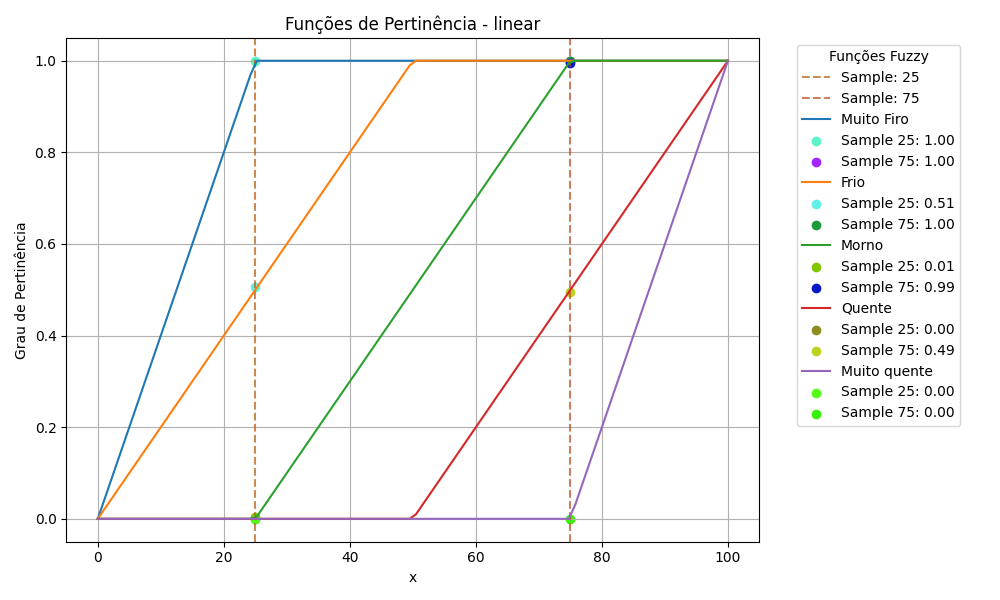
\includegraphics[width=0.8\textwidth]{img/funções_de_pertinência_linear_fuzzificado.png}
    \caption{Funções de pertinência sigmoidais e graus de ativação.}
\end{figure}
Ativações para o tipo gaussian:

Ativações para o tipo linear:
Samples: [25, 75]
Muito Firo: [1, 1]
Frio: [0.51, 1.0]
Morno: [0.01, 0.99]
Quente: [0.0, 0.49]
Muito quente: [0, 0]



\section{Operações Fuzzy}

\subsection{Complemento, União e Interseção}

\subsubsection{Complemento:}

Zadeh
\begin{verbatim}    
    def complemento_zadeh(u):
    return 1 - np.array(u)
\end{verbatim}

Sugeno:
\begin{verbatim}    
    def complemento_sugeno(u, lamb=0.5):
    return (1 - u) / (1 + lamb * u)
\end{verbatim}


Yager:
\begin{verbatim}    
    def complemento_yager(u, w=2):
    return (1 - u**w)**(1/w)
\end{verbatim}

\subsubsection{União (t-conormas):}
Máximo
\begin{verbatim}    
    def complemento_yager(u, w=2):
    return (1 - u**w)**(1/w)
\end{verbatim}

Soma Probabilística
\begin{verbatim}
def uniao_soma_probabilistica(u1, u2):
    return u1 + u2 - u1 * u2
\end{verbatim}


Soma Limitada
\begin{verbatim}
def uniao_soma_limitada(u1, u2):
    return np.minimum(1, u1 + u2)
\end{verbatim}

Soma Drástica
\begin{verbatim}
def uniao_soma_drastica(u1, u2):
    return np.where((u1 == 0) & (u2 == 0), 0, np.maximum(u1, u2))
\end{verbatim}



\subsubsection{Interseção (t-conormas)}
Mínimo
\begin{verbatim}
def intersecao_minimo(u1, u2):
    return np.minimum(u1, u2)
\end{verbatim}

Produto
\begin{verbatim}
def intersecao_produto(u1, u2):
    return u1 * u2
\end{verbatim}


Produto Limitado
\begin{verbatim}
def intersecao_produto_limitado(u1, u2):
    return np.maximum(0, u1 + u2 - 1)
\end{verbatim}

Produto Drástico
\begin{verbatim}
def intersecao_produto_drastico(u1, u2):
    return np.where((u1 == 1) & (u2 == 1), np.minimum(u1, u2), 0)
\end{verbatim}

\subsection{Relaçõess Fuzzy}



Este relatório apresentou a definição, particionamento e análise de funções de pertinência para a variável temperatura ambiente. A análise gráfica e textual destacou as diferenças entre os tipos de funções, evidenciando suas características e aplicações.



\end{document}